\chapter{Exercise 2}
The purpose of this exercise is to understand the various method of setting up
the virtual camera and to be able to adjust the parameters of the camera. We will
get more acquainted with defining the matrices in the viewing pipeline and to
concatenate them into the viewing matrix. Secondly, we will make different
pictures of the scene using various projection method based on central projection
(Front, X and 3-point perspective) and Orthographic parallel projection
(Isometric, Dimetric, and Trimetric axonometric).


\section{Part 1}
\begin{itemize}
\item Vertex structure in Exercise 1 was represented by a pair of 2D cartesian coordinates
as vec2 and a color as vec3. On the other hand in Exercise 2 vertices are points in
3D space so they are represented in homogenous coordinates as vec4.
\item In Exercise 1 in display function we defined an Ortho2D projection and we were describing
model-view properties of our vision. In this exercise we use Ortho (3D) projection and we use
a LookAt function which takes an eye position, an up vector, and look at positon, which does
a camera inverse transformation (creates a modelView matrix).
\end{itemize}
\clearpage

\section{Part 2}
To produce a required output I used 3 transformations in an order:
\begin{enumerate}
\item Translation
\item Scaling
\item Rotation around Y axis
\end{enumerate}
\begin{lstlisting}[language=cpp, caption={Transformations}]
modelView *= Angel::Translate(0,3,0);
modelView *= Angel::Scale(2,2,2);
modelView *= Angel::RotateY(30);
\end{lstlisting}
An output for this order of transformation can be seen in Figure \ref{fig:exercise_2_part_2},
however if we change the order of transformations for example make Translate the last operation,
we can get different output, because matrix multiplication isn't a commutative operation.
\begin{figure}[ht!]
	\begin{center}
		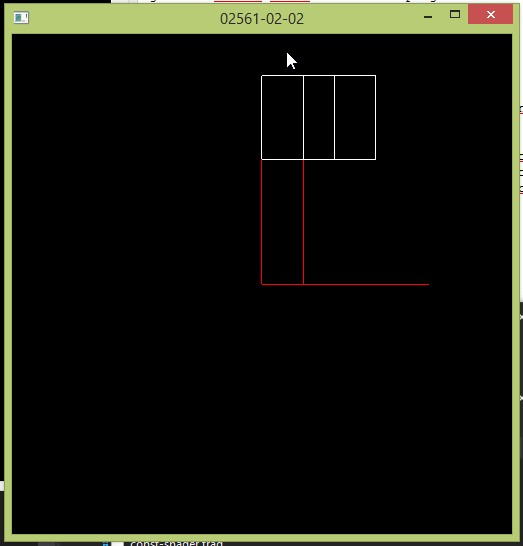
\includegraphics[width=0.5\textwidth]{figures/exercise_2_part_2}
	\end{center}
	\caption{Exercise 2 part 2 output}
	\label{fig:exercise_2_part_2} 
\end{figure}
\clearpage


\section{Part 3}
Following the instructions in the exercise part 2 gave me an expected result which can be seen below:
\begin{figure}[ht!]
	\begin{center}
		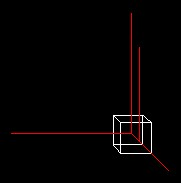
\includegraphics[width=0.5\textwidth]{figures/exercise_2_part_3}
	\end{center}
	\caption{Exercise 2 part 3 output}
	\label{fig:exercise_2_part_3} 
\end{figure} \\
To aquire this I used the following code:
\begin{lstlisting}[language=cpp, caption={Front perspective projection}]
mat4 projection = Angel::Perspective(45, 1, 1, 100);
glUniformMatrix4fv(projectionUniform, 1, GL_TRUE, projection);
vec3 eye(20, 5, 5);
vec3 up(0, 1, 0);
vec3 at(0, 5, 5);
mat4 modelView = Angel::LookAt(eye, at, up);//*Angel::Scale(3,3,3);
\end{lstlisting}
\clearpage


\section{Part 4}
I succeeded in creating an isometric view using code below, the results are shown in Figure \ref{fig:exercise_2_part_4}
\begin{lstlisting}[language=cpp, caption={Front perspective projection}]
mat4 projection = Ortho(-6., 6., -6., 6., -6., 10.);
glUniformMatrix4fv(projectionUniform, 1, GL_TRUE, projection);
vec3 eye(5,5,5);
vec3 at(0,0,0);
vec3 up(0,0,1);
mat4 modelView = Angel::LookAt(eye, at, up);
\end{lstlisting}
\begin{figure}[ht!]
	\begin{center}
		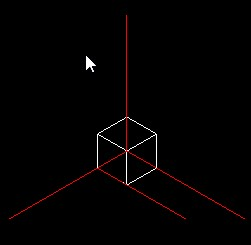
\includegraphics[width=0.5\textwidth]{figures/exercise_2_part_4}
	\end{center}
	\caption{Exercise 2 part 4 output}
	\label{fig:exercise_2_part_4} 
\end{figure}



\section{Part 5}
I managed to get the same results using corresponding code parts:
\begin{lstlisting}[language=cpp, caption={Rotation and translation 1}]
// view = LookAt(vec4(-.5, 1, 6,1), vec4(-2,1,0,1), vec4(0,1,0,0));
view = RotateY(-atan(1.5/6.0)/DegreesToRadians) * Translate(.5, -1, -6);
\end{lstlisting}
\begin{lstlisting}[language=cpp, caption={Rotation and translation 2}]
// view = RotateY(-120) * Translate(-4, -1, -1);
vec3 eye(4, 1, 1);
vec3 at(4-sqrt(3), 1, 2);
vec3 up(0,1,0);
view = LookAt(eye, at, up);
\end{lstlisting}
\begin{lstlisting}[language=cpp, caption={Rotation and translation 3}]
// view = LookAt(vec4(-1, 1, 9,1), vec4(-1,1,0,1), vec4(0,1,0,0));
view = mat4(
	1,0,0,0,
	0,1,0,0,
	0,0,1,0,
	1,-1,-9,1
	);
\end{lstlisting}


\section{Part 6}
\begin{description}
  \item[Part 1 transformation]
  	$$\emph{Angel::RotateX(atan(3/6)/DegreesToRadians)*Angel::Translate(0,-3,-6);}$$
  \item[Part 2 transformation]
  	$$\emph{Angel::Translate(0,3,0)*Angel::RotateY(30)*Angel::Scale(2,2,2);}$$
\end{description}
